\documentclass[12pt]{article}
\usepackage{fullpage, amsfonts, amsmath, amsthm, amssymb, array, enumerate, systeme, wasysym, graphicx}
\usepackage[margin=0.75in]{geometry}


\begin{document}
\pagestyle{empty}



\begin{center} \textbf{\large MA 630 Collaboration Problems for Module 1} 

\vspace{.15in}
\textbf{\large Group 3}

\vspace{.25in}

\textbf{Authors} %list the full names of all authors below this line in a comma separated list
\\Bailey Koebrick, Adam Frank

\end{center}

\begin{enumerate}
\item The following is a theorem and a potential proof. Evaluate the proof for clarity and correctness. If you find any mistakes, identify them, and then provide a correct proof.\\\\
\textbf{Theorem.} If $m$ is an even integer and $n$ is an odd integer, then $5m + 3n$ is odd.\\\\
\emph{Proof.} Let $m$ be an even integer and $n$ an odd integer. Then, by definition, $m = 2k$ and $n = 2k + 1$ for some integer $k$. Thus,
\begin{align*}
5m + 3n & = 5 (2k) + 3 (2k + 1)\\
& = 10 k + 6k + 3\\
& = 16 k + 3\\
& = 2(8 k + 1) + 1.
\end{align*}
Thus, since $8k + 1$ is an integer, $5m + 3n$ is odd. \qed

% Solution by Adam Frank

{\it Evaluation.}  The proof is clear and reaches a true conclusion, although there is a logical error.  We cannot assume that $m=2k$ and $n=2k+1$ using the same value $k$ in each.  We should replace $k$ with $k_1$ and $k_2$.  Also it can increase clarity if we create a symbol for $5k_1+3k_2+1$.

{\it Corrected proof.}  Let $m$ be an even integer and $n$ an odd integer. Then, by definition, $m = 2k_1$ and $n = 2k_2 + 1$ for some integers $k_1$ and $k_2$. Thus,
\begin{align*}
5m + 3n & = 5 (2k_1) + 3 (2k_2 + 1)\\
& = 10 k_1 + 6k_2 + 3\\
& = 2(5k_1+3k_2) + 3\\
& = 2(5k_1+3k_2+1) + 1.
\end{align*}
Thus, since $5k_1+3k_2+1$ is an integer, call it $t$, then we have $5m+3n = 2t+1$.  Thus $5m + 3n$ is odd. \qed

%Solution by Bailey Koebrick
\item The following is a theorem and a potential proof. Evaluate the proof for clarity and correctness. If you find any mistakes, identify them, and then provide a correct proof.\\\\
\textbf{Theorem.} Let $n$ be an integer. If $3n - 8$ is odd, then $n$ is odd.\\\\
\emph{Proof.} For $n$ to be odd, it must be the case that $n = 2k + 1$ for some integer $k$. Therefore,
\[3n - 8 = 3 (2k + 1) - 8 = 2 (3k - 3) + 1.\]
Since $3k - 3$ is an integer, it must be that $3n - 8$ is odd, which completes the proof. \qed

{\it Evaluation.}  The proof is clear and reaches a true conclusion following the method of a direct proof. However, the proof does not follow the logical flow of the initial proposition. The initial proposition is of the form $P \rightarrow Q$ but the proof follows the form of $Q \rightarrow P$.  

{\it Corrected proof.} Let $n$ be an integer. If $3n - 8$ is odd, then $n$ is odd.\\\\
\emph{Proof.} For $n$ to be odd, it must be the case that $3n - 8 = 2k + 1$ for some integer $k$. \\

Therefore,
\begin{align*}
        3n - 8 &= 2k + 1\\
    2n + n - 8 &= 2k + 1\\
            n &= 2k - 2n + 9\\
            n &= 2k - 2n + 8 + 1\\
            n &= 2(k - n + 4) + 1\\
\end{align*}
Since $(k - n + 4)$ is an integer, it must be that $n$ is odd, which completes the proof. \qed




\item The following is a theorem and a potential proof. Evaluate the proof for clarity and correctness. If you find any mistakes, identify them, and then provide a correct proof. First, a definition.\\\\
\textbf{Definition.} Two integers, $a$ and $b$, are said to be of the \emph{same parity} if either
\begin{itemize}
\item $a$ and $b$ are both even, or
\item $a$ and $b$ are both odd.
\end{itemize}
\textbf{Theorem.} Let $x$ and $y$ be integers. Then $x + y$ is even if and only if $x$ and $y$ are of the same parity.\\\\
\emph{Proof.} We proceed by cases.\\
\textit{Case 1. $x$ and $y$ are both even:} Then \[x + y = 2k + 2l = 2(k + l),\] and thus $x + y$ is even.\\
\textit{Case 2. $x$ and $y$ are both odd:} Then \[x + y = (2k + 1) + (2l + 1) = 2k + 2l + 2 = 2(k + l + 1),\] and therefore $x + y$ is even.\\
\textit{Case 3. $x$ is even and $y$ is odd:} Then \[x + y = 2k + (2l + 1) = 2k + 2l + 1 = 2(k + l) + 1,\] and therefore $x + y$ is odd.\\
\textit{Case 4. $x$ is odd and $y$ is even:} Then \[x + y = (2k + 1) + 2l = 2k + 2l + 1 = 2(k + l) + 1,\] and therefore $x + y$ is odd.\\
Since we have exhausted all possible cases, the theorem is proved. \qed

% Solution by Adam Frank

{\it Evaluation.}  The proof could be clearer if we state in advance that $x=2k$ where $k$  is an integer, and likewise for $y$.  And likewise for the case when they're odd.  

Also the proof could be made more clear by making explicit the part which demonstrates the ``if'' portion of the claim and which demonstrates the ``only if'' portion.

However there is no fundamental logical mistake--the proof is correct, even if done while skipping some explanation.

{\it Corrected proof.}  Suppose $x$ and $y$ are integers.  To begin with we prove that if $x$ and $y$ are of the same parity then $x+y$ is even.  We proceed in this direction by cases.

{\it Case 1.} Suppose $x$ and $y$ are both even.  Let $x=2k$ and $y=2l$ for some integers $k$ and $l$.  Then 

\begin{align*}
    x+y = 2k+2l = 2(k+l)
\end{align*}

Since $k+l$ is an integer, call it $t$, then $x+y=2t$ is an even number.

{\it Case 2.}  $x$ and $y$ are both odd.  Let $x=2k+1$ and $y=2l+1$ for some integers $k$ and $l$.  Then 

\begin{align*}
    x+y = 2k+1+2l+1 = 2(k+l+1)
\end{align*}

Since $k+l+1$ is an integer, call it $t$, then $x+y=2t$ is an even number.

Since the result holds in all cases, we have finished this direction.  Now for the converse we will prove this by its contrapositive.  That is to say we will prove that if $x$ and $y$ are not of the same parity then $x+y$ is not even.  So assume $x$ and $y$ are not of the same parity, and again we have two cases.

{\it Case 3.} $x$ is even and $y$ is odd.  Let $x=2k$ and $y=2l+1$ for integers $k$ and $l$.  Then 

\begin{align*}
    x+y = 2k+2l+1 = 2(k+l)+1
\end{align*}

Since $k+l$ is an integer, call it $t$, then $x+y=2t+1$ is not an even number.

{\it Case 4.} $x$ is odd and $y$ is even.  Let $x=2k+1$ and $y=2l$ for integers $k$ and $l$.  Then 

\begin{align*}
    x+y = 2k+1+2l = 2(k+l)+1
\end{align*}

Since $k+l$ is an integer, call it $t$, then $x+y=2t+1$ is not an even number.

Again this result holds in all cases and so we have proved this direction.  \qed


%Solution by Bailey Koebrick
\item Below is the (correct) proof of some result. Identify the result being proved. Be sure to justify your response.\\\\
\textbf{Theorem.} ... Let $x, y$ and $z$ be integers. If $xy$ is even, then $xy + yz + xz$ must also be even.\\

{\it Justification.} By reading through the proof, we can identify that the ultimate goal is to prove $xy + yz + xz$ must be even and to do so, it must be assumed that the variables used, $x, y,$ and $z$ are integer values. Lastly, we look at why "we may assume that $x$ and $y$ are even". If $xy$ were to equal an even integer, we could conclude that $x$ and $y$ might also be even integers as the product of two even integers is an even integer.

\emph{Proof.} Without loss of generality, we may assume that $x$ and $y$ are even. Then $x = 2a$ and $y = 2b$ for some integers $a$ and $b$. Thus,
\[xy + yz + xz = (2a)(2b) + (2b)z + (2a)z = 2(2ab + bz + az),\]
and therefore $xy + yz + xz$ is even. \qed





\item Below is the (correct) proof of some result as well as a missing step in the proof. Identify the result being proved, and complete the missing paragraph of the proof. Be sure to justify your response.\\\\
\textbf{Theorem.} ...\\\\
\emph{Proof.} [Missing paragraph]\\\\
First, assume that $3x - 2$ is even. Thus, $x$ is even, and hence $x = 2a$ for some integer $a$. Thus,
\[5x + 1 = 5 (2a) + 1 = 10a + 1 = 2(5a) + 1,\]
and therefore $5x + 1$ is odd.\\
Now, assume that $3x - 2$ is odd. Thus, $x$ must be odd, and therefore $x = 2b + 1$ for some integer $b$. Thus,
\[5x + 1 = 5(2b + 1) + 1 = 10 b + 6 = 2(5b + 3),\]
and therefore $5x + 1$ is even.



\item \textbf{Definition.} A prime number is called \emph{average} if it is the average of two \emph{different} prime numbers (e.g. $7 = \dfrac{11 + 3}{2}$, and hence 7 is an average prime). Consider the following propositions:
\begin{itemize}
\item[] $P$: Every prime greater than 3 is average.
\item[] $Q$: Every positive, even integer other than 2 can be written as the sum of two primes (which are possibly the same). (Goldbach's conjecture)
\item[] $R$: Every even integer greater than 6 can be written as the sum of two \emph{different} prime numbers. 
\end{itemize}
It is believed that $P$, $Q$, and $R$ are all true, but proofs have not been discovered. However, it is readily shown that if $P$ and $Q$ are both true, then $R$ is true, and vice versa. Prove that $(P \wedge Q) \leftrightarrow R$.




\item The following is a collection of four ``proofs without words'' (of course, these are not \emph{proofs}) of the same result. For each image below, identity the result and then provide a rigorous, mathematical proof of the result.
\begin{center}
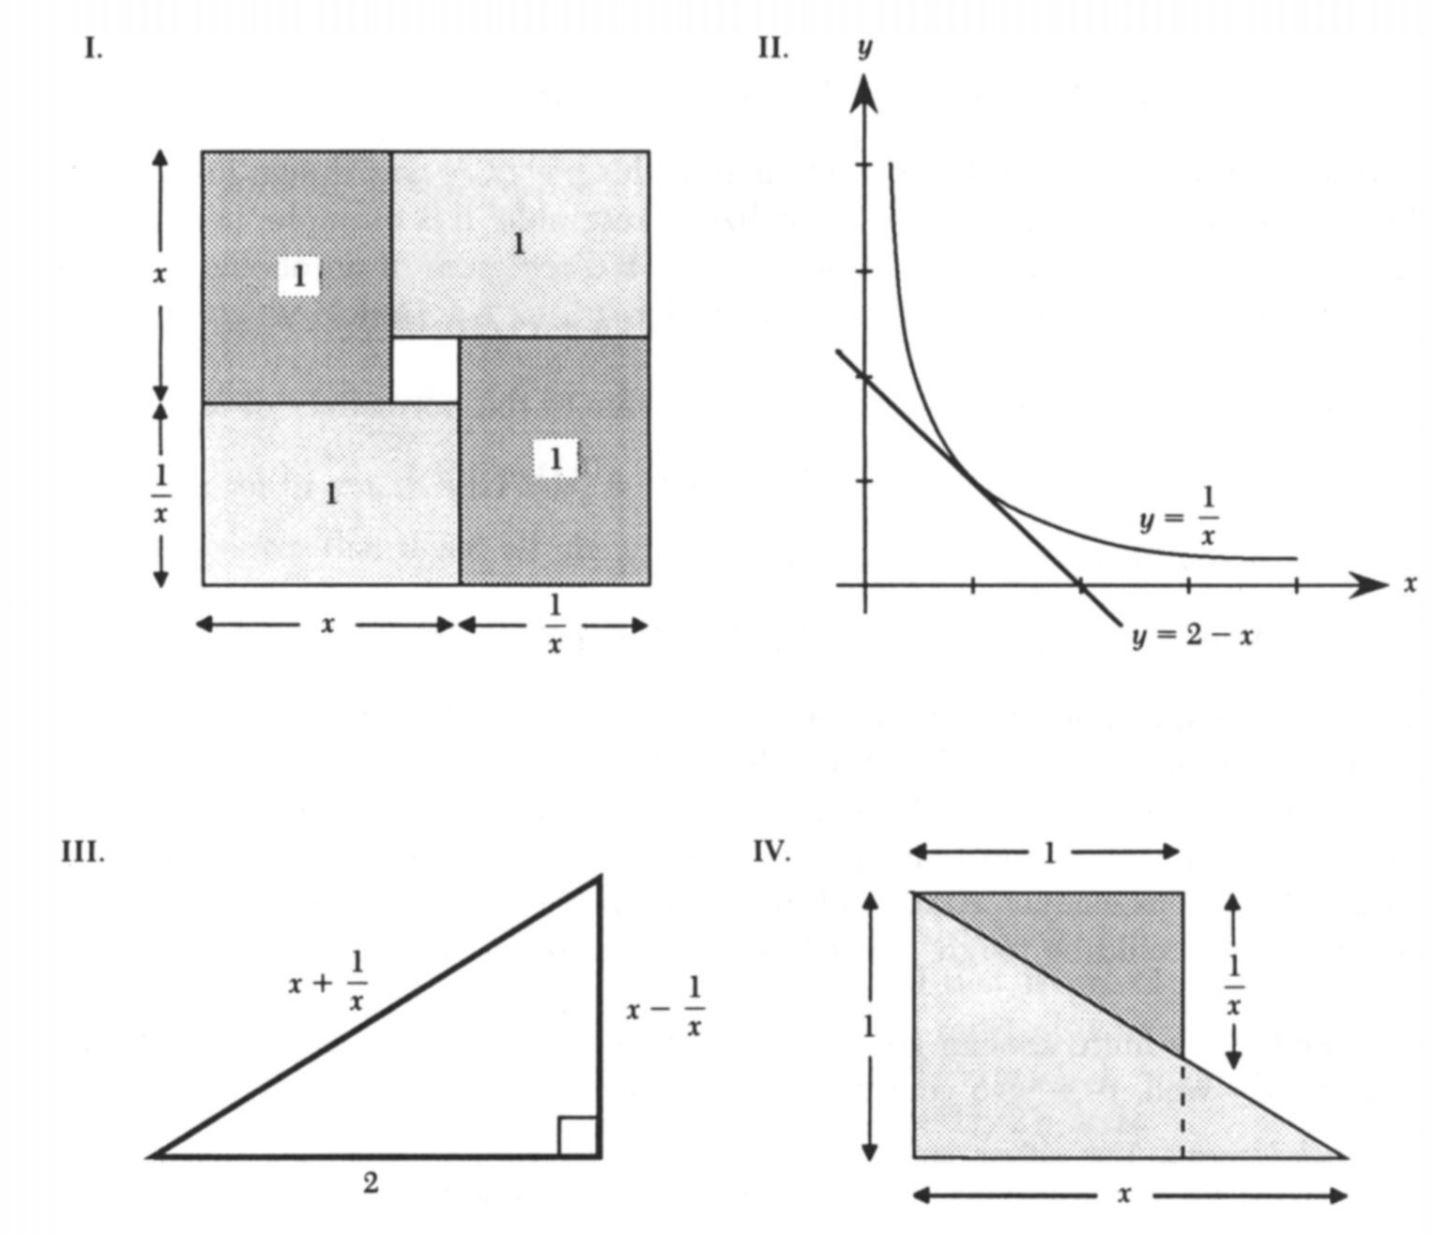
\includegraphics[scale=0.4]{pww_1.jpg}
\end{center}
%Solution by Bailey Koebrick
II. \emph{Proof.} When graphed in the $xy$ plane, $y=\frac{1}{x}$ and $y=2-x$ intersect when $x=1$.

If $y=\frac{1}{x}$ and $y=2-x$ intersect when $x=1$, it can be assumed that each equations respective $y$ values will also be equal.

Therefore,
\begin{align*}
     \frac{1}{x} &= 2 - x\\
               1 &= 2x - x^2\\
    x^2 - 2x + 1 &= 0\\
  (x - 1)(x - 1) &= 0\\
\end{align*} 
where the solution is x = 1. This proves the original proposition to be true.\\

%Solution by Bailey Koebrick
III. \emph{Proof.} There exists a right-triangle with sides $a$, $b$ and hypotenuse $c$, where $a=2$, $b=x-\frac{1}{x}$ and $c=x+\frac{1}{x}$, such that $a^2 + b^2 = c^2$ for all $x \in \mathbb R$, so long as $x \ne 0$.

Therefore,
\begin{align*}
     a^2 + b^2 &= c^2\\\\
     (2)^2 + (x-\frac{1}{x})^2 &= (x+\frac{1}{x})^2\\\\
     4 + (x-\frac{1}{x})(x-\frac{1}{x}) &= (x+\frac{1}{x})(x+\frac{1}{x})\\\\
     4 + x^2 - 1 - 1 + \frac{1}{x^2} &= x^2 + 1 + 1 + \frac{1}{x^2}\\\\
     x^2 + \frac{1}{x^2} + 2 &= x^2 + \frac{1}{x^2} + 2\\
\end{align*} 
Because is can be assumed that $x=x$, both sides of the equation are logically equivalent proving the original proposition to be true for all $x \in \mathbb R$ so long as $x \ne 0$.
\end{enumerate}
\end{document}